\documentclass[12pt]{article}
\usepackage{graphicx}
\usepackage{xcolor}
\usepackage{subfigure}
\usepackage[margin=1.0in]{geometry}
\usepackage{float}
\usepackage{amsmath}
\usepackage{mathtools}
\usepackage{wrapfig}
\usepackage{setspace}
\usepackage{multicol}
\renewcommand{\baselinestretch}{1.5}
\usepackage[utf8]{inputenc}
\usepackage{etoolbox}
\patchcmd{\thebibliography}{\section*{\refname}}{}{}{}
\usepackage{sectsty}
\sectionfont{\fontsize{12}{15}\selectfont}
\subsectionfont{\fontsize{12}{15}\selectfont}
\usepackage{titlesec}
\titlespacing*{\section}{0pt}{0.2\baselineskip}{0.2\baselineskip}
\titlespacing*{\subsection}{0pt}{0.2\baselineskip}{0.2\baselineskip}
\setlength{\abovedisplayskip}{0pt}
\setlength{\belowdisplayskip}{0pt}
\usepackage{etoolbox}
\patchcmd{\thebibliography}
  {\settowidth}
  {\setlength{\itemsep}{0pt plus 0.01pt}\settowidth}
  {}{}
\apptocmd{\thebibliography}
  {\small}
  {}{}
\author{Shivesh Pathak}
\title{Developing effective theories for single and bilayer graphene using density matrix downfolding}

\begin{document}
\maketitle
\begin{abstract}
Building accurate model Hamiltonians for realistic materials is a fundamental problem in modern condensed matter physics.
A recently developed density matrix downfolding (DMD) \cite{Zheng2017} method provides a very direct framework for downfolding the \textit{ab initio} Hamiltonian to a many-body effective Hamiltonian using only \textit{ab initio} calculations. 
Here I propose a two year thesis plan for developing atomic scale many-body model Hamiltonians for single- and simple bi-layer graphene systems within the DMD framework using high accuracy \textit{ab initio} quantum Monte Carlo (QMC) calculations.
The results of my thesis will lay the groundwork for a continuing four year project to build a twist dependent many-body continuum model for the twisted bilayer graphene (TBLG) system.
To demonstrate my preparedness I present a model Hamiltonian developed using DMD which accurately reproduces the spectra and properties of the lowest lying excitations of the CuO molecule.
\end{abstract}
Committee: Lucas Wagner, Brian DeMarco, Andre Schleife, Karin Dahmen
\pagebreak

\section{Introduction}
Developing model Hamiltonians for realistic materials is a fundamental problem in modern condensed matter physics.
A model Hamiltonian is a simplified description of a real material which can accurately reproduce the low-lying eigenstates and energies of the material.
Accurate models give clear and direct indications of effective interactions within a material and underpin modern theoretical understanding of ideas like emergence and symmetry breaking.
On a practical level, calculations related to these low-lying eigenstates can be carried out on the much simpler model and still yield accurate results reflective of reality.

Yet unresolved is a paradigm for building many-body model Hamiltonians which can describe strongly correlated systems.
Band and Fermi liquid theory have been successful in accurately modeling systems where effective interactions are negligible at low energy scales.
These theories, however, fail in describing the low-energy excitations of strongly correlated systems like high Tc superconductors and TBLG.
Minimal many-body models like the Hubbard \cite{Hubbard1963}, Kanamori \cite{10.1143/PTP.30.275}, t-J \cite{Chao_1977} and Heisenberg models have been proposed to describe such systems, their effectiveness in describing realistic materials is unclear.

In an attempt to build accurate many-body Hamiltonians for realistic systems, a framework for model development using solutions from \textit{ab initio} simulations has emerged.
Common approaches involve density functional theory (DFT) \cite{PhysRev.140.A1133, PhysRevLett.87.047003} alongside random phase approximation (RPA) or other methods \cite{PhysRevB.62.R16219, PhysRevB.70.195104, PhysRevB.88.075106}.
L\"owdin methods and canonical transformations have also been used to develop effective theories \cite{doi:10.1063/1.4802766, PhysRevA.81.013402, doi:10.1063/1.2196410}.
While useful, it is typically impossible to know whether models built from these techniques accurately describe reality, as measures of model quality are rarely reported.
Instead, comparisons of model predictions to experiment are conducted for model validation.

The recently developed DMD \cite{Zheng2017} method provides a more direct link between \textit{ab initio} and many-body effective Hamiltonians.
Similar to the methods above, DMD uses information from \textit{ab initio} simulations on the system to fit the best parameters for a given many-body model \textit{ansatz}.
Unlike the methods above, the resultant fit model is accompanied by a clear measure of model quality, quantifying the ability of the model to reproduce the low-energy spectrum of the system.
Since model quality is reported, DMD allows for direct comparison between different model \textit{ansatzes} as well, an ability which can be used to deduce important model terms using \textit{ab initio} calculations.
DMD has been used to develop accurate many-body models for benzene, a 1-d hydrogen chain, and an on-site Hubbard model for graphene \cite{Zheng2017, Wagner2015}.

The utility of DMD is made apparent when studying the recent surge in model development for TBLG.
\textit{ab initio} model development has so far been restricted to tight-binding models which accurately describe single particle effects like band flattening, but do not address interactions \cite{Fang, Fang2016, PhysRevX.8.031088, PhysRevX.8.031087}.
Minimal interacting models have been proposed using traditional theoretical methods, but without a link to \textit{ab initio} it is unclear whether they can describe the real system \cite{PhysRevB.98.045103, PhysRevB.100.125116, PhysRevX.8.031089}.
DMD can bridge the gap between these methods by providing a framework to build an accurate many-body model directly from \textit{ab initio} simulations on TBLG.

As such, a project named QMC High Accuracy Multiscale Modeling (QMC HAMM) between research groups at UIUC, UCSB and Rice University is dedicated towards the development of an accurate continuum-scale interacting model for TBLG.
The model development consists of two layers of downfolding: first, developing an atomic scale lattice model using \textit{ab initio} calculations, and second, downfolding the resultant lattice model to a continuum length scale.
My thesis will be focused on the first layer of downfolding.
I propose a two year plan for developing many-body lattice models for single- (SLG) and simple bi-layer (BLG) graphene systems using the DMD method and \textit{ab initio} fixed-node diffusion Monte Carlo (FN-DMC) calculations.
My thesis will lay the necessary ground work for the development of a fully twist angle dependent lattice model for TBLG, and an eventual continuum model.

\subsection{Density Matrix Downfolding (DMD)}
I begin by defining what a low-energy effective Hamiltonian and downfolding are.
Consider a high-energy Hamiltonian $\hat{H}$ and Hilbert space $\mathcal{H}$.
A low-energy effective Hamiltonian is an operator $\hat{H}_\text{eff}$ which can accurately reproduce the spectra and eigenstates of $\hat{H}$ on a subpsace $\mathcal{LE}$ of the Hilbert space $\mathcal{H}$.
Here $\mathcal{LE}$ is the span of the N lowest energy eigenstates of $\hat{H}$, and $\hat{H}_\text{eff}$ is a linear combination of Hermitian operators $\hat{d}_k$ with a constant shift $E_0$
\begin{equation}
\hat{H}_\text{eff} = \sum_{k} g_k \hat{d}_k  + E_0.
\label{eq:Heff}
\end{equation}
The objective of Hamiltonian downfolding is to construct such an $\hat{H}_\text{eff}$ given $\hat{H}, \mathcal{H}$.

The key insight of DMD is that the Hamiltonian downfolding problem can be mapped onto a linear regression problem.
It has been shown \cite{Zheng2017} that the above definition of $\hat{H}_\text{eff}$ is equivalent to the following: a low-energy effective Hamiltonian is an operator such that 
\begin{equation}
\begin{split}
\forall |\Psi\rangle \in \mathcal{LE},\ E[\Psi] = E_\text{eff}[\Psi]  + \epsilon[\Psi]
\end{split}
\label{eq:DMD}
\end{equation}
where $\epsilon[\Psi]$ is the error in the effective theory and the energy functionals are defined as $E[\Psi] \equiv \langle \Psi | \hat{H} |\Psi \rangle,\  E_\text{eff}[\Psi] \equiv \langle \Psi | \hat{H}_\text{eff} |\Psi \rangle$.
Given the general linear form of $\hat{H}_\text{eff}$ seen in \eqref{eq:Heff}, 
the task of building an effective Hamiltonian then reduces to fitting a linear model that minimizes the error $\epsilon[\Psi]$ over $\mathcal{LE}$.
The independent variables (descriptors) in the fitting are expectation values of the operators $d_k[\Psi] \equiv \langle \Psi |\hat{d}_k|\Psi \rangle$ and the target variable is $E[\Psi]$.

This linear regression problem can be tackled in three steps.
First, low-energy states are sampled from $\mathcal{LE}$.
Next, a pool of candidate operators $\{\hat{d}_k\}$ which may be included in the final model are selected.
Finally, a linear regression is carried out with descriptor and energies evaluated on the sampled states as the independent and target variables.

When developing models for realistic system, $\hat{H}$ is taken to be the \textit{ab initio} Hamiltonian
\begin{equation}
\hat{H}_\text{ab} = \sum_i -\frac{1}{2} \nabla_i^2 + \sum_{iI}\frac{Z_I}{|r_i - R_I|} + \frac{1}{2} \sum_{ij} \frac{1}{|r_i - r_j|} + E_\text{ion}(\{R_I\})  
\label{eq:Hab}
\end{equation} 
where index $i,j$ correspond to electrons, $I$ to ions, and $E_\text{ion}$ corresponds to the ionic kinetic and potential energies. 
The unit of energy is Hartree (Ha).
To reduce the computational expense of \textit{ab initio} calculations one works under the Born-Oppenheimer approximation where $E_\text{ion}$ becomes a constant.
Ionic effects related to phonon modes can be recovered by altering the ionic geometry and observing the effects on the electronic state.

Low-energy states can be accessed using any wave function based \textit{ab initio} simulation technique, but two broad principles are used for selecting a method.
First, the method should be able to generate accurate low-energy wave functions in the \textit{ab initio} Hilbert space, as the accuracy of the low-energy states dictate the accuracy of the final model.
Second, the method should be relatively inexpensive, as large amounts of training data are preferred for a more robust regression.
QMC methods have typically been selected due to their polynomial scaling computational cost and high accuracy, but DFT can also be used as an initial step trading accuracy for computational ease.

Candidate descriptors are typically selected using both physical intuition and statistical methods.
An essential first pass involves selecting a large set of descriptors using knowledge of the low-energy degrees of the freedom of the system and physical principles like symmetry.
Further filtering follows by examining the relationship between descriptors and the \textit{ab initio} energy over the low-energy sampled states: descriptors will typically be discarded if they do not exhibit covariance with the energy.
Note, while there is no restriction on the form of the candidate operators other than Hermiticity, 1- and 2-body second quantized operators are commonly used.

A standard fitting workflow involves feature selection, model regression and model validation.
Feature selection methods for choosing descriptors from the candidate pool can range from wrapper methods like principal component analysis \cite{pearson_karl_1901_1430636} to regularized embedded methods like LASSO \cite{10.2307/2346178}. 
Fitting the effective Hamiltonian usually involves an ordinary least squares linear regression, but the cost function can be altered.
Model validation can be carried out by calculating cross validated single parameter measures like $R^2$ scores which carry information about goodness of fit and overfitting.

The results of the linear regression are an estimate of the parameter values $g_k$ and model error $\epsilon[\Psi]$.
The error estimate usually takes the form of a goodness of fit, such as a cross-validated $R^2$ score or root mean squared error (RMSE).
These error estimates present a direct measurement of model quality, ensuring that DMD not only gives the best fit parameters but also an assessment of model validity.
Further, by quantifying model quality through statistical error estimates, it is possible to compare the accuracy of various low-energy \textit{ansatzes}.

\subsection{Fixed-node diffusion Monte Carlo (FN-DMC)}
Diffusion Monte Carlo (DMC) is a QMC method which projects out the ground state of a real-space Hamiltonian given some initial trial wave function.
Consider a trial wave function $|\Psi_T\rangle$ and the Hamiltonian $\hat{H}$ with ground state $|\Phi_0\rangle$. 
Applying the projector $e^{-\tau \hat{H}}$ as $\tau \rightarrow \infty$ to $|\Psi_T \rangle$
\begin{equation}
\lim_{\tau \rightarrow \infty} e^{-\tau \hat{H}} |\Psi_T\rangle 
\equiv \lim_{\tau \rightarrow \infty} |\Psi_\text{DMC}(\tau)\rangle \propto \langle \Phi_0|\Psi_T\rangle |\Phi_0\rangle,
\end{equation}
projects out the ground state as long as the trial wave function is not orthogonal to the ground state. 
DMC provides a stochastic implementation of the projection by moving samples from $\Psi_T(R)$ using the Green function $G(R, R^\prime, \tau) = \langle R | e^{-\tau(\hat{H} - E_T)} | R^\prime \rangle$, which is approximated using a Trotter expansion $G(R, R^\prime, \tau) \sim \Big[e^{-d\tau(\frac{V(R) + V(R^\prime)}{2} - E_T)} \langle R| e^{-d\tau\hat{T}}|R^\prime \rangle + O(d\tau^2) \Big]^N $ 
where $d\tau = \tau/N$.
This expansion can be interpreted as an interative procedure where samples are moved N times with a small timestep $d\tau$ until convergence.
The constant $E_T$ is a trial energy used to control the normalization of $\Psi_\text{DMC}(\tau, R)$ and is updated at each move.

DMC, however, suffers from a fermion sign problem which is alleviated via a fixed-node approximation.
Under the fixed-node approximation the nodal surface of $\Psi_\text{DMC}(\tau, R)$ is forced to match that of the initial trial wave function for all $\tau$.
This approximation makes FN-DMC variational, and will only return the exact ground state of $\hat{H}$ if the nodal surfaces of $|\Psi_T\rangle$ and $|\Phi_0\rangle$ are identical.

While seemingly disadvantageous, the variational nature of FN-DMC plays
a key role in generating the low-energy states needed for DMD.
Consider a set of trial wave functions with varying nodal structures.
The final projected $\Psi_\text{DMC}$ for these different trial functions will be the lowest energy states in $\mathcal{H}$ for the given nodal structures.
If the initial trial wave functions are appropriately chosen, the final projected states will be within the target low-energy subspace of $\mathcal{H}$.

The training data required for downfolding are extracted from the projected low-energy states via a mixed estimator.
Due to the fixed-node approximation, the final distribution returned by the projection is $f(R) = \Psi_T(R) \Psi_\text{DMC}$, and Monte Carlo estimates of operator expectation values correspond to the mixed estimation $\frac{\langle \Psi_T | \hat{O} | \Psi_\text{DMC} \rangle}{\langle \Psi_T | \Psi_\text{DMC}\rangle}$. 
This does not equal the target expectation value $\frac{\langle \Psi_\text{DMC} | \hat{O} | \Psi_\text{DMC} \rangle}{\langle \Psi_\text{DMC} | \Psi_\text{DMC}\rangle}$, resulting in a mixed estimator error.
Details on alleviating this error in DMD and evaluation of expectation values for 1- and 2-body second quantized operators can be found in the literature \cite{Wagner2015, Wagner2017}.
\section{Preliminary Work}
\subsection{Non-orthogonal determinants in FN-DMC trial wave functions}
In order to become acquainted with QMC algorithms I worked on implementing and testing multi-Slater-Jastrow trial functions with optimized non-orthogonal determinants (MSJ+NO) in FN-DMC \cite{doi:10.1063/1.5052906}.
The MSJ+NO trial wave functions take the form
\begin{equation}
\Psi=e^{J(\vec{\alpha})} \sum_I e^{\hat{\Theta}(\vec{\theta_I})} C_I |D_I (\{ \phi\})\rangle
\end{equation}
where the determinants $|D_I\rangle$ are composed of single particle orbitals from a self-consistent field calculation, $e^J$ is a spin-independent Jastrow factor, and $e^{\hat{\Theta}}$ is a spin-dependent orbital rotation matrix.
The wave function has variable parameters $\vec{\alpha}, \vec{\theta}, \vec{C}$ which can be optimized.

I assessed the efficiency and compactness of the new function by calculating the ground state energy of a C$_2$ molecule using FN-DMC and comparing to the results when using multi-Slater-Jastrow trial functions with orthogonal determinants (MSJ+O). 
The workflow involved constructing the un-optimized trial wave functions, optimizing the parameters using an energy optimization method \cite{Toulouse2007}, and finally using the optimized trial functions in FN-DMC calculations. 
The average improvement in the FN-DMC energy with the MSJ+O trial wave functions was $\langle E_{MSJ} - E_{MSJ,O}\rangle =$ 0.14eV with an additional reduction of 0.032 eV when using the MSJ+NO trial wave function.
While the benefit using the MSJ+NO trial wave function seems small, the energy calculated using an MSJ+NO trial function with only 24 determinants was lower than the energy using an MSJ+O trial 
function with 55 determinants.

Further, the FN-DMC charge density calculated using MSJ+NO trial functions had stronger bonding character than when using MSJ+O trial functions, a reasonable result as introducing correlations into trial functions allows for electrons to avoid each other while still occupying the same bonding region. 
The results indicated that using non-orthogonal determinants may lead to more compact trial wave functions for small molecules.

\subsection{Effective theory for CuO molecule using DMD}
To become acquainted with DMD, I constructed a many-body effective model for the CuO molecule with fixed bond length $r_e$ = 1.725\r{A}.
In the following three sections I will detail the steps I took towards developing a model for the CuO molecule using DMD, followed by a comparison of model spectra to experiment.

\vspace{-10pt}
\paragraph{Sampling low-energy states}
For the CuO molecule, low-energy states were generated by using FN-DMC projected multi-Slater-Jastrow (MSJ) trial wave functions.
The trial wave functions took the form
\begin{equation}
|\Psi_T(\vec{p}) \rangle =  e^{J}\sum_{j} p_j|\text{D}_j\rangle,
\label{eq:sampling}
\end{equation}
where $e^J$ is a Jastrow factor, $|\text{D}_j\rangle$ are selected determinants, and $p_j$ are variable coefficients.
By varying $\{p_j\}$ one can move around the low-energy space if the set $\{|\text{D}_j \rangle\}$ is representative of the low-energy excitations in the system.
The Jastrow factor explicitly introduces electronic correlation and reduces the localization error within FN-DMC \cite{Foulkes2001}.

The determinants $|\text{D}_j \rangle$ were constructed from the orbitals of independent symmetry-targeted unrestricted Kohn Sham (UKS) calculations.
This choice was made to ensure that the three major low-energy variations seen in the molecule were captured: occupancy, spin configuration and relaxation of the Cu 3d, 4s and O 2p orbitals.
Only determinants with electrons in the Cu 3d, 4s, and O 2p orbitals and at most a single hole in the Cu 3d shell were included in \eqref{eq:sampling} to reflect the low-energy excitations seen in experiment.
The UKS calculations were done using PySCF \cite{Sun2018}, a B3LYP functional \cite{doi:10.1063/1.464304, PhysRevB.37.785}, Trail-Needs psuedopotential and VTZ Trail-Needs basis \cite{doi:10.1063/1.4811651}.

A shell sampling scheme was used to select coefficients $p_j$ for the trial wave functions.
We began by fixing the coefficient $p_0 = \sqrt{w}$ where $w \in \{1.0, 0.8, ..., 0.2\}$. 
For each choice of $w$, n = 5 states were selected by sampling the unassigned coefficients from independent, standard normal distributions such that $\sum_j p_j^2 = 1$. 
This procedure generated a uniform set of samples from spherical shells at decreasing radii in determinant space centered at $|\text{D}_0\rangle$.
The process was repeated by centering at every determinant in \eqref{eq:sampling}, resulting in a sample set of overlapping shells which fill the low-energy space.

A single three-body Jastrow factor was used for all trial wave functions, and was optimized on the lowest energy determinant $|\text{D}_0 \rangle$ using an energy optimization scheme \cite{Toulouse2007}.
This choice significantly reduced the computational cost of sampling low-energy states as linear optimization was not necessary for every sampled state.
The resulting MSJ trial function remained low in energy as variations of the Jastrow factor among low-energy states is expected to be small.

The sampled MSJ trial wave functions were projected using FN-DMC to generate the final set of low-energy sample states.
FN-DMC calculations were conducted with T-moves \cite{PhysRevB.74.161102} to ensure the variational principle holds while using pseudopotentials, and a timestep of $\tau = 0.01$.
All QMC calculations were done in QWalk \cite{Wagner2009}.

\vspace{-10pt}
\paragraph{Selecting candidate descriptors}
The following set of 1- and 2-body operators were selected as candidates for the model based on an understanding of the low-energy excitations of the CuO molecule and properties of the sampled low-energy states:
\begin{equation}
\begin{split}
\sum_{\sigma = \uparrow, \downarrow} \Bigg(\epsilon_{3d_\pi}\hat{n}_{3d_\pi,\sigma} + \epsilon_{3d_{z^2}}\hat{n}_{3d_{z^2},\sigma} +  \epsilon_{2p_z} \hat{n}_{2p_z,\sigma} + \epsilon_{2p_\pi}\hat{n}_{2p_\pi,\sigma} + \epsilon_{4s}\hat{n}_{4s,\sigma} +
t_\pi \hat{c}_{3d_\pi,\sigma}^\dagger \hat{c}_{2p_\pi,\sigma} + t_{dz} \hat{c}_{3d_{z^2},\sigma}^\dagger \hat{c}_{2p_z,\sigma}\\
  + t_{sz}\hat{c}_{4s,\sigma}^\dagger \hat{c}_{2p_z,\sigma} + t_{sd}\hat{c}_{4s,\sigma}^\dagger \hat{c}_{3d_{z^2},\sigma} + \text{h.c.} \Bigg)  +
J_{sd}\sum_{i\in {\{\text{xy, xz, ...}}\}} \vec{S}_{4s} \cdot \vec{S}_{3d_i} + U_s \hat{n}_{4s,\uparrow}\hat{n}_{4s,\downarrow} + E_0.
\end{split}
\label{eq:models}
\end{equation}
The operator subscripts correspond to the intrinsic atomic orbital (IAO) basis elements constructed using the molecular orbitals in \eqref{eq:sampling}, and can be seen in \ref{fig:cuo_regr}a.

The first chunk of descriptors were selected using physical intuition and symmetry principles.
As described above, the low-lying excitations in CuO observed in experiment involve the Cu 3d, 4s and O 2p atomic orbitals.
Given that orbitals also hybridize, the occupation energies of and hopping terms between these orbitals were selected as candidate operators.
Symmetry considerations help narrow down the set as hopping terms are only non-zero between same symmetry orbitals, and occupation energies can be traced over symmetry related orbitals, for example $n_{2p_\pi} = n_{2p_x} + n_{2p_y}$.
The term $\sum_{i\in {\{\text{xy, xz, ...}}\}} \vec{S}_{4s} \cdot \vec{S}_{3d_i}$ was also considered, motivated by the existence of a $\sim $0.5 eV Hund's coupling observed on the copper atom \cite{Data2009}.

The inclusion of a double occupancy term $n_{4s,\uparrow} n_{4s,\downarrow}$ was motivated directly from the sampled low-energy states.
Within the sampled data, states with a Cu $4s^{2}$ configuration lie at least 7 eV above the lowest energy sampled state, while the lowest energy state with a $4s^{1}$ configuration lies at 1.6 eV.
If the double occupancy term was not included, the effective theory would predict the prior state to have an energy of $\sim $ 3eV, an underestimation of 4 eV from the \textit{ab initio} result.
The effective on-site Coulomb repulsion $U_s$ ensures the model places all such $4s^{2}$ states high in energy.

\begin{figure*}
\centering
%\hspace*{-0.25in}
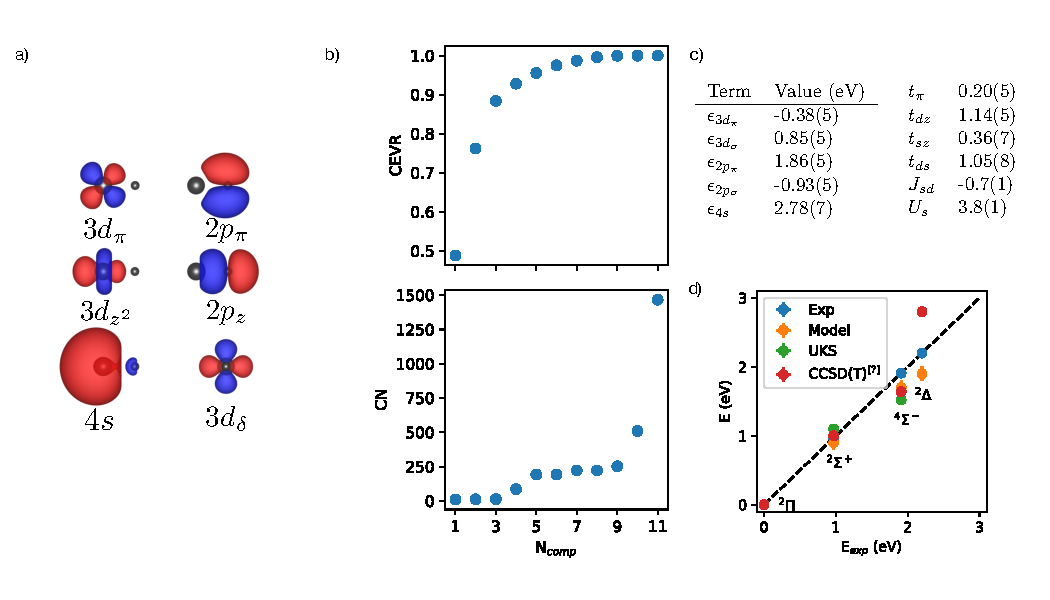
\includegraphics[width=1.0\linewidth]{./figs/cuo_regr_2.pdf}
\caption{Figures related to model regression for the CuO molecule: a) Intrinsic atomic orbitals used as a single particle basis for the model Hamiltonian, b) Results of PCA showing the CEVR and CN of a data set containing N$_{comp}$  highest ranked PCs, c) The final regressed parameters from the PCR, d) Comparison of four lowest lying eigenstates of CuO molecule between experiment and three computation methods.}
\label{fig:cuo_regr}
\end{figure*}

\vspace{-10pt}
\paragraph{Fitting the model}
A direct attempt at fitting all eleven terms in \eqref{eq:models} leads to a high goodness of fit, R$^2$ = 0.99, but unexpectedly large coefficients for the fit model.
This is seen in an enormous occupation energy gap of $\epsilon_{2p_\pi} - \epsilon_{3d_\delta} = $ 5.87 eV, which is 2 $-$ 3 eV in experiment and our sampled data.
This inflation of model parameters was found to be associated with multicollinearity among the candidate descriptors, quantified by a large condition number (CN) of 1470.

A principal components analysis (PCA) on the descriptors illustrates the multicollinearity in the data set.
In Figure \eqref{fig:cuo_regr}b I show the cumulative explained variance ratio (CEVR) and CN of a matrix composed of the $N_\text{comp}$ highest ranked PCs varying from one to eleven.
The CEVR indicates how much of the variation in the descriptor values a subset of PCs capture, and the CN quantifies the multicollinearity among these PCs.
The sharp decrease in the condition number and sustained high CEVR up to nine principal components indicates the presence of only nine linearly independent variations within the descriptor set.

To reduce multicollinearity while maintaining a high goodness of fit, a model was fit to these nine PCs.
When trained on all the sampled data this model yields an $R^2$ = 0.98 with a CN of 257. 
An inverse PCA transformation was used to map the fit coefficients corresponding to the PC descriptors back into the original eleven coefficients of \eqref{eq:models}.
These coefficients can be seen in Figure \ref{fig:cuo_regr}c with single standard deviation bootstrap error estimates.
The procedure carried out here is well established and called principal components regression (PCR) \cite{10.2307/2348005}.

\vspace{-10pt}
\paragraph{Solutions of the model}
The final model in \ref{fig:cuo_regr}c was solved by exact diagonalization, and the solutions agree well with experimental spectra and state assignments.
Shown in Figure \ref{fig:cuo_regr}d is a comparison between the excitation energies calculated from the model and those seen in the latest anion photoelectron spectroscopy measurements \cite{Wu1997}.
The model energies for these eigenstates are denoted by orange circles and agree with experiment up to a maximum deviation of 0.2 eV.
Further, the term symbols assigned in experiment match the term symbols of the model eigenstates, which are constructed by looking at the multiplicity and electronic configuration of each model eigenstate. 

The energies for the UKS and CCSD(T) \cite{Xian2000} states are also shown in Figure \ref{fig:cuo_regr}d as green and red circles, respectively.
The UKS energies were calculated in this work in en route to constructing the determinants $|\text{D}_j\rangle$ used in our sampling scheme \eqref{eq:sampling}.
The model energies agree with both theoretical techniques within errorbars for the first three states shown.
The energy of the highest energy $^2\Delta$, however, is severely over estimated using both UKS and CCSD(T), by nearly 1 eV.
This over estimation may arise from an inadequate relaxation of the $\sigma$ type orbitals which form a three orbital hybridization complex in this system.

\section{Proposed work}
I propose a two year thesis plan for developing atomic scale many-body
model Hamiltonians for SLG and simple BLG systems within the DMD framework using high accuracy \textit{ab initio} QMC calculations.
To do so, I will be building a sequence of four many-body model Hamiltonians for increasing complex systems: the benzene molecule, SLG, AA stacked BLG, and AB stacked BLG.
The following sections detail the sampling scheme and candidate models that will be used for downfolding each system.
I conclude with a brief statement about the impact of my work within the QMC HAMM project and modeling TBLG and a timeline.

\subsection{Constrained variational Monte Carlo (cVMC)}
A new constrained cVMC method will be used to sample the low-energy wave functions necessary for DMD.
The cVMC method works by minimizing the following cost function for a parameterized wave function $|\Psi(\vec{p})\rangle$:
\begin{equation}
\vec{p}^* = \text{argmin} \ \langle \Psi(\vec{p}) | \hat{H}_\text{ab} | \Psi(\vec{p}) \rangle - \sum_k [\lambda_k \langle \Psi(\vec{p}) | d_k - d_{k}^0 | \Psi(\vec{p}) \rangle]^2
\end{equation}
with respect to the parameters $\vec{p}$.
The quantity $\vec{d}$ is short hand for a list of candidate descriptors to sample variations in, $\vec{d}^*$ is the target values of those descriptors, and $\vec{\lambda}$ controls the importance of finding a state with low-energy versus one with descriptor values near $\vec{d}^*$.
This method allows one to target low-energy wave functions which sit near a target point $\vec{d}^*$ in descriptor space, allowing for a more systematic sampling of the low-energy space.

I will use a multi-Slater-Jastrow (MSJ) parameterization in the cVMC sampling.
The multi-Slater expansion will consist of determinants of single particle orbitals calculated using DFT.
Given the nature of graphene-like systems, as described below, the determinants will include the DFT ground state as well as molecular orbital excitations among the $\pi$ and $\pi^*$ orbitals which form the active space.
A three body Jastrow factor will be applied to ensure that correlations are included in the wave function and that the wave function is low in energy.
The total set of parameters $\vec{p}$ will be Jastrow and determinental coefficients.

\subsection{Benzene}
The first system I will develop a model for is the benzene molecule, shown in Figure \ref{fig:proposed}a.
While relatively simple, this molecule shares many similarities with and forms the basic unit of SLG.
The delocalized $\pi$ orbitals in benzene carry over directly into SLG where they are the primary contributors to the well known Dirac bands.
Interaction effects seen in the benzene molecule are also reflected in SLG, such as on-site double occupation energies for the carbon atoms \cite{Zheng2017, Wagner2015}.

\begin{figure*}
\centering
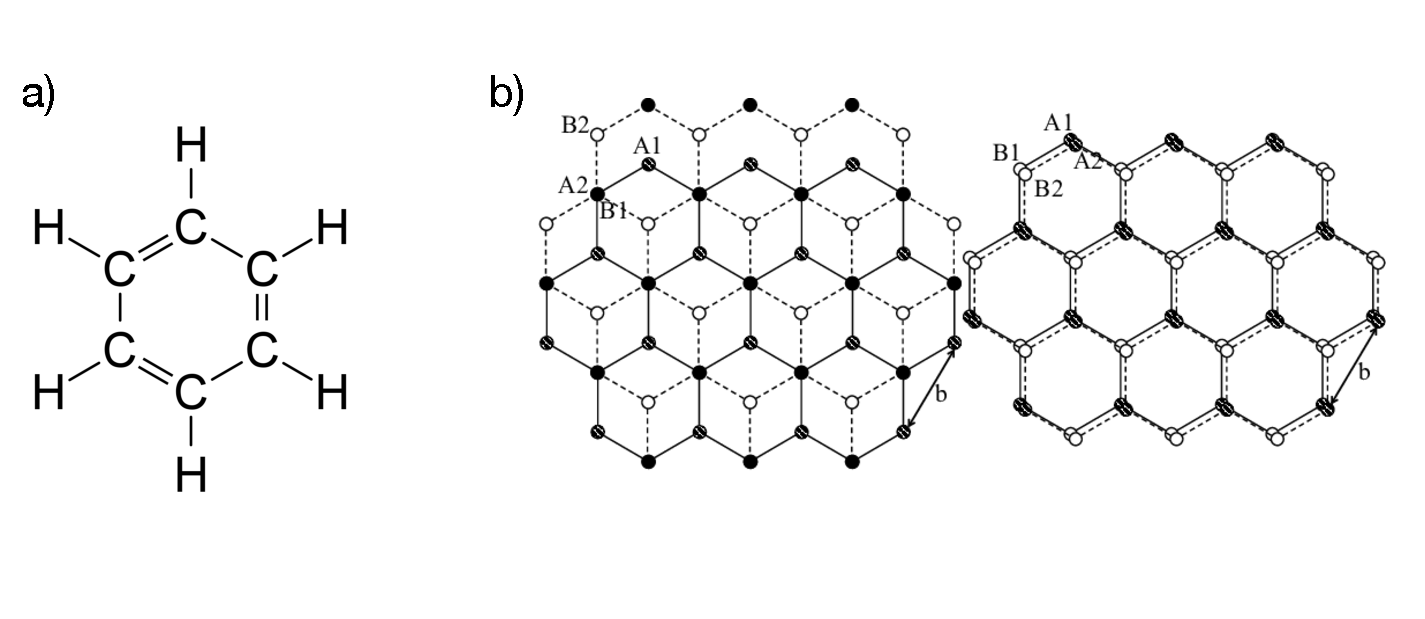
\includegraphics[width=1.0\linewidth]{./figs/proposed.pdf}
\caption{Schematic diagrams for the a) benzene molecule, b) AB and AA stacked BLG \textbf{ref}.}
%Voltage Tunable Plasmon Propagation in Dual Gated Bilayer Graphene
\label{fig:proposed}
\end{figure*}

My objective will be to reproduce a previously developed many-body model for the benzene molecule using QMC DMD \cite{Wagner2015}.
In this study, an extended Hubbard model built on the six $\pi$ orbitals was found to perform well in describing the low-lying excitations of the material.
The final model took the form 
\begin{equation}
H_\text{benz} = -\sum_{\langle i,j \rangle} t_{ij}c_i^\dagger c_j + U \sum_i n_{i\uparrow}n_{i\downarrow}  + \sum_{\langle i,j \rangle}V_{ij} n_i n_j + \sum_{\langle \langle i,j \rangle\rangle}V_{ij} n_i n_j
\label{Hbenz}
\end{equation}
where the brackets denote nearest neighbor and next-nearest neighbor summations.
As such, the model \textit{ansatz} that I will try to fit will be \eqref{Hbenz}.

This first stage of model development provides a playground for benchmarking new model fitting procedures.
Downfolding techniques have advanced significantly since the initial model for benzene was developed in 2015.
Methods like constrained VMC for low-energy sampling have been posited but not thoroughly tested.
By comparing models built using new methods directly to the 2015 model, it will be possible to quantify the efficiency and effectiveness of these methods.

\subsection{SLG}
The second system I will work on is SLG.
Single layer graphene is composed of a triangular Bravais lattice with two carbon atoms per unit cell.
In terms of a non-interacting picture, the $\sigma$ orbitals composed of C $2s, 2p_x,$ and $2p_y$ lie below the Fermi level.
The bands which cross the Fermi level, and compose the distinct Dirac cones seen in SLG, are primary $\pi$ bonded molecular orbitals composed of C $2p_z$ orbitals.
Further, reduced screening in SLG leads to long range Coulomb interactions in the system \cite{Elias2012, Yu2013}.

I will work on extending an on-site Hubbard model for SLG \cite{Zheng2017, Wagner2015} to one with long-range Coulomb interactions.
The candidate model will be of the form:
\begin{equation}
H_\text{SLG} = -\sum_{i,j} t_{ij}c_i^\dagger c_j + U \sum_i n_{i\uparrow}n_{i\downarrow}  + \sum_{i,j} V_{ij} n_i n_j
\label{Hslg}
\end{equation}
where the indices correspond to the $\pi$ orbitals on the copper atoms.
I will consider both long range hopping and density-density interaction terms extending across the computational unit cell, with the final goal of developing position dependent parameter values $t(r), V(r)$.

The resultant model will be able to non-parametrically determine the form
of long-range interactions in graphene.
This is an important contribution to the study of interaction effects in graphene as many potential properties of the system depend on details of these long-range interactions.
Such effects include edge magentism \cite{PhysRevB.95.195420} and non-local electrodynamics \cite{PhysRevB.90.045137}.

\subsection{BLG}
The last systems I will develop models for are AA and AB stacked BLG, shown in Figure \ref{fig:proposed}b.
AA stacked BLG is simply two sheets of graphene placed on top of one another where each atom is aligned with the atom beneath it.
In AB stacked BLG, a carbon atom from the lower layer is present in the center of each carbon hexagon of the upper layer, and vice versa.
As such, one can think of AB BLG as a shifted version of AA BLG, where the shift is half the size of a single carbonic hexagon.

I anticipate that the candidate descriptors should include interlayer couplings as well as the terms seen in SLG.
As such, the candidate model for BLG would be
\begin{equation}
H_\text{BLG} = H_\text{SLG}^{(1)} + H_\text{SLG}^{(2)} - \sum_{i_1, i_2} t_{i_1, i_2}^\prime c_{i_1}^\dagger c_{i_2} + h.c.
\label{Hblg}
\end{equation}
There are two terms for the single layers from \eqref{Hslg} plus an interlayer hopping given by the term $t_{i_1, i_2}^\prime.$  
The index $i_1$ refers to layer 1 and $i_2$ to layer two.
While this is an initial \textit{ansatz}, additional inter- and intra-layer terms can be included if necessary.

With these two models, one can begin to answer some prominent questions about the inter-layer coupling in TBLG.
First, one can determine, at least for the simplest orientations, whether the inter-layer coupling takes the form of a hopping or interaction term.
While current studies tend to assume the prior \cite{Fang, Fang2016, PhysRevX.8.031088, PhysRevX.8.031087}, there is no good reason to discount the latter.
Further, the quantitative details of spatial dependence, which are intimately related to the strongly correlated behavior in TBLG, can begin to be addressed.

\vspace{-10pt}
\paragraph{QMC HAMM}
A major goal of the QMC HAMM project is to develop a twist dependent, Moire length scale, interacting model for TBLG using QMC \textit{ab initio} calculations.
The first step in doing so is developing an atomic scale model for TBLG, and the necessary prerequisites for this step are a strong understanding of effective theories of the basic constituents of the system.
The models I propose to develop for SLG and AA/AB BLG provide exactly this kind of understanding.
As such, my work will lay the foundation for the four year QMC HAMM project to build an effective theory for TBLG.

\vspace{-10pt}
\paragraph{Proposed timeline} I believe that developing effective theories for the benzene molecule, SLG, AA and AB stacked BLG should take 2 years. 
The model fitting for benzene should take no more than four months as it is a reproduction of previous work.
The SLG model fitting should take another eight months.
As an extension of a previous work, the first three months will be dedicate to reproducing the on-site Hubbard model from that work.
Inclusion of long range Coulomb interactions into the effective theory should take another three months.
The last two months will be geared towards finite size extrapolation in order to ensure the final model is applicable to bulk systems.
The last year of the project will be focused on the AA and AB BLG, with each project taking six months to complete.
For each stacking, need four months to build the model and two months for finite size extrapolation.


\vspace{-10pt}
\begin{multicols}{2}
\begin{spacing}{0.5}
{\footnotesize
\bibliography{biblio}
\bibliographystyle{prelim}
}
\end{spacing}
\end{multicols}
\end{document}
